
%(BEGIN_QUESTION)
% Copyright 2015, Tony R. Kuphaldt, released under the Creative Commons Attribution License (v 1.0)
% This means you may do almost anything with this work of mine, so long as you give me proper credit

\noindent
{\bf Lab Exercise -- introduction}

\vskip 5pt

Your task is to build, document, and troubleshoot a flow measurement system consisting of a ``smart'' electronic differential pressure transmitter connected to an electronic indicator, recorder, or indicating controller.  Air flow and water flow are suggested process variables to measure.  Alternatives to the standard flow-measurement lab are authorized by instructor permission only.

The following table of objectives show what you and your team must complete within the scheduled time for this lab exercise.  Note how some of these objectives are individual, while others are for the team as a whole:

\underbar{Objective completion table:}

% No blank lines allowed between lines of an \halign structure!
% I use comments (%) instead, so that TeX doesn't choke.

$$\vbox{\offinterlineskip
\halign{\strut
\vrule \quad\hfil # \ \hfil & 
\vrule \quad\hfil # \ \hfil & 
\vrule \quad\hfil # \ \hfil & 
\vrule \quad\hfil # \ \hfil & 
\vrule \quad\hfil # \ \hfil & 
\vrule \quad\hfil # \ \hfil & 
\vrule \quad\hfil # \ \hfil \vrule \cr
\noalign{\hrule}
%
% First row
{\bf Performance objective} & {\bf Grading} & {\bf 1} & {\bf 2} & {\bf 3} & {\bf 4} & {\bf Team} \cr
%
\noalign{\hrule}
%
% Another row
Prototype sketch ({\it before building the system!}) & mastery & -- & -- & -- & -- & \cr
%
\noalign{\hrule}
%
% Another row
Circuit design challenge & mastery & & & & & -- -- -- -- \cr
%
\noalign{\hrule}
%
% Another row
Final loop diagram and system inspection & mastery & & & & & -- -- -- -- \cr
%
\noalign{\hrule}
%
% Another row
Spreadsheet characterizing flow element & mastery & -- & -- & -- & -- &  \cr
%
\noalign{\hrule}
%
% Another row
Flow/DP prediction ($\pm$ 5\% of span) & mastery & & & & & -- -- -- -- \cr
%
\noalign{\hrule}
%
% Another row
Troubleshooting & mastery & & & & & -- -- -- -- \cr
%
\noalign{\hrule}
%
% Another row
Lab question: Instrument connections & proportional &  &  &  &  & -- -- -- -- \cr
%
\noalign{\hrule}
%
% Another row
Lab question: Commissioning & proportional &  &  &  &  & -- -- -- -- \cr
%
\noalign{\hrule}
%
% Another row
Lab question: Math & proportional &  &  &  &  & -- -- -- -- \cr
%
\noalign{\hrule}
%
% Another row
Lab question: Diagnostics & proportional &  &  &  &  & -- -- -- -- \cr
%
\noalign{\hrule}
%
% Another row
Decommission and lab clean-up & mastery & -- & -- & -- & -- &  \cr
%
\noalign{\hrule}
} % End of \halign 
}$$ % End of \vbox

The only ``proportional'' scoring in this activity are the lab questions, which are answered by each student individually.  A listing of potential lab questions are shown at the end of this worksheet question.  The lab questions are intended to guide your labwork as much as they are intended to measure your comprehension, and as such the instructor may ask these questions of your team day by day, rather than all at once (on a single day).

\vskip 10pt

{\bf It is essential that your team plans ahead what to accomplish each day.  A short (10 minute) team meeting at the beginning of each lab session is a good way to do this, reviewing what's already been done, what's left to do, and what assessments you should be ready for.  There is a lot of work involved with building, documenting, and troubleshooting these working instrument systems!}

As you and your team work on this system, you will invariably encounter problems.  You should always attempt to solve these problems as a team before requesting instructor assistance.  If you still require instructor assistance, write your team's color on the lab whiteboard with a brief description of what you need help on.  The instructor will meet with each team in order they appear on the whiteboard to address these problems.

$$\includegraphics[width=15.5cm]{i00490x01.eps}$$




\vfil \eject

\noindent
{\bf Lab Exercise -- selecting components and planning the system}

\vskip 5pt

One of the most common problems students encounter when building any working system, whether it be a circuit on a solderless breadboard or an instrument loop spanning an entire room, is properly connecting and configuring all components.  An unfortunate tendency among most students is to simply start connecting parts together, essentially designing the system as they go.  This usually leads to improperly-connected components and non-functioning systems, sometimes with the result of destroying components due to those improper connections!

An alternative approach is to plan ahead by designing the system before constructing it.  This is easily done by sketching a diagram showing how all the components should interconnect, then analyzing that diagram and making changes before connecting anything together.  When done as a team, this step ensures everyone is aware of how the system should work, and how it should go together.  The resulting ``prototype'' diagram need not be complex in detail, but it should be detailed enough for anyone to see which component terminals (and ports) connect to terminals and ports of other devices in the system.  For example, your team's prototype sketch should be clear enough to determine all DC electrical components will have the correct polarities.  If your proposed system contains a significant amount of plumbing (pipes and tubes), your prototype sketch should show all those connections as well.

\vskip 10pt

Your first step should be selecting proper field instruments from the instrument storage area to use in building your system.  In this particular lab, you are looking for a ``smart'' differential pressure transmitter which you will use to measure the pressure drop across a flow element such as a Pitot tube, orifice plate, or venturi tube.  The Rosemount model 1151 smart, 3051, or 3095 transmitters are appropriate for this application.  You should choose a differential pressure transmitter with a measurement range that can turn down to approximately 10 inches water column.  Avoid high-range transmitters (ranges exceeding 10 PSI or so).  The maximum pressure range of the transmitter you select depends on the turndown (``rangedown'') of that transmitter.  If the transmitter has a large turndown (e.g. 100:1), then you might be able to get away with using one calibrated from the factory with a high range (e.g. 0 to 40 PSI).  

You will also need to locate a valve manifold to isolate the transmitter from the process pressure.  Either a three-valve or a five-valve manifold will work well for this purpose.

The next step should be finding appropriate documentation for your differential pressure transmitter.  Nearly every instrument in the lab is documented electronically at the manufacturer's website, so your best resource is the Internet (and/or your Instrumentation Reference where a variety of instrument manuals have been downloaded for you).  Use this documentation to identify how to properly connect and calibrate the transmitter.  Your instructor will check to see you have located and are familiar with the equipment manual(s).

After locating a suitable instrument and its associated documentation, you should qualitatively test it prior to installing it in your system.  For a pressure transmitter, this entails applying an air pressure to the ``high'' pressure port and measuring the transmitter's milliamp output signal to see if it responds to the application of pressure.  If the transmitter fails to respond properly, tag it with a label explaining what it does (or what it fails to do).

\vskip 10pt

Your team's prototype sketch is so important that the instructor will demand you provide this plan before any construction on your team's working system begins.  {\it Any team found constructing their system without a verified plan will be ordered to cease construction and not resume until a prototype plan has been drafted and approved!}  Each member on the team should have ready access to this plan (ideally possessing their own copy of the plan) throughout the construction process.  Prototype design sketching is a skill and a habit you should cultivate in school and take with you in your new career.

\vskip 10pt

{\bf Planning a functioning system should take no more than an hour if the team is working efficiently, and will save you hours of frustration (and possible component destruction!).}







\vfil \eject

\noindent
{\bf Lab Exercise -- circuit design challenge}

\vskip 5pt

Your instructor will choose one 4-20 mA field instrument and one control system from the lists shown below, for which you must sketch an accurate circuit diagram showing how the two instruments would connect to each other.  If this interconnection between controller and field instrument requires additional electrical components to function (e.g. DC or AC power source, precision 250 $\Omega$ resistor, diode, relay, etc.), those must be incorporated into your diagram as well.  Instruction manuals for all instrument listed are available on the electronic Instrumentation Reference for your convenience.  When your sketch is complete, you must show the relevant manual pages to your instructor for verification of correct connections.

This exercise tests your ability to locate appropriate information in technical manuals and sketch a correct 4-20 mA loop circuit for a given pair of instruments.  The electronic Instrumentation Reference will be available to you in order to answer this question.

\vskip 10pt

Since all 4-20 mA ``loops'' are basically series DC circuits, it is highly recommended that you approach their design the same as for any other DC circuit: carefully identify all {\it sources} and {\it loads} in the circuit, trace directions of all currents, and mark the polarities of all voltages.  Most of the mistakes made in this type of circuit design challenge may be remedied by careful consideration of these specific circuit-analysis details.


%%%%%%%%%%%%%%%%%%%%%%%%%%%%%%%
\vskip 10pt
\filbreak
\hbox{ \vrule
\vbox{ \hrule \vskip 3pt
\hbox{ \hskip 3pt
\vbox{ \hsize=5in \raggedright

\noindent \centerline{\bf 4-20 mA transmitter options}
\item{} Pressure
\itemitem{} Rosemount 1151 Alphaline (analog), 1151 HART, or 3051 HART
\itemitem{} Yokogawa DPharp EJX110A or EJX910 
\itemitem{} Honeywell ST3000
\vskip 2pt
\item{} Level
\itemitem{} Rosemount APEX non-contact radar, 3300 GWR, or 5300 GWR
\vskip 2pt
\item{} Temperature
\itemitem{} Rosemount 444, 644, 3044, or 3144
\itemitem{} Foxboro RTT15 or RTT30
\itemitem{} Moore Industries SPT with sourcing (4-wire) 4-20 mA output
\itemitem{} Moore Industries SPT with sinking (2-wire) 4-20 mA output
\itemitem{} Moore Industries TRX or TDY
%\itemitem{} Honeywell STT173
\vskip 2pt
\item{} Flow
\itemitem{} Foxboro CFT50 coriolis
\vskip 2pt
\item{} Analytical
\itemitem{} Rosemount 5081-P (pH)
\itemitem{} Daniel 700 gas chromatograph (4 analog output channels)
\itemitem{} Foxboro 876PH (pH/ORP/ISE)
\end{itemize}

} \hskip 3pt}%
\vskip 5pt \hrule}%
\vrule}
%%%%%%%%%%%%%%%%%%%%%%%%%%%%%%%




%%%%%%%%%%%%%%%%%%%%%%%%%%%%%%%
\vskip 10pt
\filbreak
\hbox{ \vrule
\vbox{ \hrule \vskip 3pt
\hbox{ \hskip 3pt
\vbox{ \hsize=5in \raggedright

\noindent \centerline{\bf Controller options}
\item{} Monolithic
\itemitem{} Siemens 352P 
\itemitem{} Siemens 353
\itemitem{} Foxboro 716C
\itemitem{} Foxboro 718TC
\itemitem{} Foxboro 762CNA 
\itemitem{} Moore Industries 535
\itemitem{} Honeywell UDC2300
\itemitem{} Honeywell UDC3500 
\vskip 2pt
\item{} Modular -- {\it you choose the appropriate I/O module}
\itemitem{} Siemens 353R 
\itemitem{} Emerson ROC800 SCADA/RTU 
\vskip 2pt
\item{} Distributed Control System (DCS) -- {\it you choose the appropriate I/O module}
\itemitem{} Emerson DeltaV with M-series I/O
\itemitem{} Emerson DeltaV with S-series I/O 
\itemitem{} Honeywell Experion with 2MLF series I/O 
\vskip 2pt
\item{} Programmable Logic Controller (PLC) -- {\it you choose the appropriate I/O module}
\itemitem{} Siemens S7-300 
\itemitem{} Rockwell ControlLogix (catalog number 1756)
\itemitem{} Rockwell CompactLogix (catalog number 1769)
\end{itemize}

} \hskip 3pt}%
\vskip 5pt \hrule}%
\vrule}
%%%%%%%%%%%%%%%%%%%%%%%%%%%%%%%




%%%%%%%%%%%%%%%%%%%%%%%%%%%%%%%
\vskip 10pt
\filbreak
\hbox{ \vrule
\vbox{ \hrule \vskip 3pt
\hbox{ \hskip 3pt
\vbox{ \hsize=5in \raggedright

\noindent \centerline{\bf 4-20 mA Final Control Element options}
\item{} Pneumatic control valve positioners
\itemitem{} Fisher 3582i positioner 
\itemitem{} Fisher DVC6000 positioner 
\vskip 2pt
\item{} Electrically actuated valves (MOV)
\itemitem{} Limitorque actuator with Modutronic-20 II controller 
\itemitem{} Rotork AQ with Folomatic controller 
\vskip 2pt
\item{} AC motor drives (VFD)
\itemitem{} Rockwell PowerFlex 4 
\itemitem{} Automation Direct GS1 
\end{itemize}

} \hskip 3pt}%
\vskip 5pt \hrule}%
\vrule}
%%%%%%%%%%%%%%%%%%%%%%%%%%%%%%%


\vfil

Study reference: the ``Analog Electronic Instrumentation'' chapter of {\it Lessons In Industrial Instrumentation}, particularly the section on HART.

\vskip 10pt

Note: a very effective problem-solving strategy for determining how to connect different components together to create a working 4-20 mA current loop is to first identify whether each component acts as a {\it source} or a {\it load} in that loop circuit.  Then, label voltage polarities (+ , $-$) and directions of current accordingly.  Knowing which way current must flow through each component and which polarity each voltage must have is key to ensuring the inter-component connections are correct.







\vfil \eject

\noindent
{\bf Lab Exercise -- building the system}

\vskip 5pt

The Instrumentation lab is set up to facilitate the construction of working instrument ``loops,'' with over a dozen junction boxes, pre-pulled signal cables, and ``racks'' set up with 2-inch vertical pipes for mounting instruments.  The only wires you should need to install to build a working system are those connecting the field instrument to the nearest junction box, and then small ``jumper'' cables connecting different pre-installed cables together within intermediate junction boxes.

After getting your prototype sketch approved by the instructor, you are cleared to begin building your system.  Transmitters attach to 2-inch pipes using special brackets and U-bolts.  These brackets and U-bolts are located along with the transmitters in the instrument storage area.  

Select a specific loop controller to act as a display indicator for your system.  Your instructor may choose the controller for your team, to ensure you learn more than one type of controller during the course of a quarter.

Finally, your flow-measurement system needs to have a loop number, so all instruments may be properly labeled.  This loop number needs to be unique, so that another team does not label their instruments and cables the same as yours.  One way to make your loop number unique is to use the equivalent resistor color-code value for your team's color in the loop number.  For example, if you are the ``Red'' team, your loop number could be ``2''. 

\vskip 10pt

{\bf Common mistakes:}

\begin{itemize}
\item{} Neglecting to consult the manufacturer's documentation for field instruments (e.g. how to wire them, how to calibrate them).
\item{} Mounting the field instrument(s) in awkward positions, making it difficult to reach connection terminals or to remove covers when installed.
\item{} Failing to tug on each and every wire where it terminates to ensure a mechanically sound connection.
\item{} Students working on portions of the system in isolation, not sharing with their teammates what they did and how.  It is important that the whole team learns all aspects of their system!
\end{itemize}

\vfil \eject

Air flow is a relatively easy variable to produce and measure using a venturi tube.  A venturi nozzle proven to work well with air flow may be fabricated out of a plastic (ABS) sewer pipe fitting.  The source of air flow may be physical motion (e.g. measuring the air speed of a moving vehicle) or an air blower:

$$\includegraphics[width=15.5cm]{i00490x03.eps}$$

A U-tube water manometer is shown for illustrative purposes only.  Your differential pressure transmitter will connect to the venturi to measure pressure instead of a manometer (although you may attach a manometer in parallel with the pressure transmitter if you wish, for direct visual indication of pressure drop!).

\vskip 10pt

When characterizing a flow element such as this (i.e. measuring how much differential pressure it produces for known quantities of flow rate), you will need to be able to vary the air flow through the nozzle in a predictable manner.  This may be done by varying the blower's speed.  Centrifugal blowers accelerate the air to a velocity approximately equal to the rim speed of the blower wheel:

$$\includegraphics[width=15.5cm]{i00490x06.eps}$$

If the blower's speed is halved, the air velocity will likewise be halved, and the corresponding pressure drop generated by the nozzle will be quartered.

\vfil \eject

If water flow is the desired variable, you may build a venturi tube that connects to a standard garden hose, then use a graduated bucket and a stopwatch to measure water flow rate for characterization purposes:

$$\includegraphics[width=15.5cm]{i00490x07.eps}$$

An alternative to using a bucket with volume markings on it (e.g. 1 gallon, 2 gallons, 3 gallons . . .) is to place the bucket on a bathroom scale and time how long it takes to accumulate a certain mass of water.

\vskip 10pt

When measuring the flow of any liquid, be careful to locate the DP transmitter {\it below} the venturi tube in order to avoid capturing air bubbles in the impulse lines.  Also, be sure to thoroughly bleed both impulse lines of air before using, in order to avoid measurement errors.

\vfil \eject

An interesting variation on the basic flow measurement lab is to include a control valve to throttle the air flow, and then set up a full PID loop control system to actually maintain air flow at specified setpoint values.  A simple piping arrangement to use a large (2 inch) control valve to produce a variable air flow is shown here:

$$\includegraphics[width=15.5cm]{i00490x04.eps}$$

In order to characterize the flow element on a system including a control valve, you will need to maintain the valve in a wide-open state while varying the vacuum cleaner's speed (using a lamp dimmer module or a Variac).  This, of course, means you will have to find some way to precisely gauge the vacuum cleaner's motor speed in order to know how much you are changing the flow rate.

\vskip 10pt

{\bf Building a functioning system should take no more than one full lab session (3 hours) if all components are readily available and the team is working efficiently!}





\vfil \eject

\noindent
{\bf Lab Exercise -- documenting the system}

\vskip 5pt

Each student must sketch their own {\it loop diagram} for their team's system, following proper ISA conventions.  Sample loop diagrams are shown in the next question in this worksheet.  These loop diagrams must be {\it comprehensive} and {\it detailed}, showing every wire connection, every cable, every terminal block, range points, etc.  The principle to keep in mind here is to make the loop diagram so complete and unambiguous that anyone can follow it to see what connects to what, even someone unfamiliar with industrial instrumentation.  In industry, loops are often constructed by contract personnel with limited understanding of how the system is supposed to function.  The loop diagrams they follow must be so complete that they will be able to connect everything properly without necessarily understanding how it is supposed to work.

Every instrument and every signal cable in your loop needs to be properly labeled with an ISA-standard tag number.  An easy way to do this is to wrap a short piece of masking tape around each cable (and placed on each instrument) then writing on that masking tape with a permanent marker.  Although no industry standard exists for labeling signal cables, a good recommendation is to label each two-wire cable with the tag number of the field instrument it goes to.  Thus, every length of two-wire cable in a flow transmitter circuit should be labeled ``FT-$x$'' (where ``$x$'' is the loop number), every flow control valve should be labeled ``FV-$x$'', etc.  Remember that the entire loop is defined by the process variable it measures: if the PV is {\it flow} then the transmitter with be a {\it F}T, the control valve will be a {\it F}V, the controller with be a {\it F}C, etc.

When your entire team is finished drafting your individual loop diagrams, call the instructor to do an inspection of the loop.  Here, the instructor will have students take turns going through the entire loop, with the other students checking their diagrams for errors and omissions along the way.  During this time the instructor will also inspect the quality of the installation, identifying problems such as frayed wires, improperly crimped terminals, poor cable routing, missing labels, lack of wire duct covers, etc.  The team must correct all identified errors in order to receive credit for their system.  

After successfully passing the inspection, each team member needs to place their loop diagram in the diagram holder located in the middle of the lab behind the main control panel.  When it comes time to troubleshoot another team's system, this is where you will go to find a loop diagram for that system!

\vskip 10pt

{\bf Common mistakes:}

\begin{itemize}
\item{} Forgetting to label all signal wires (see example loop diagrams).
\item{} Forgetting to label all field instruments with their own tag names (e.g. FT-83).
\item{} Forgetting to note all wire colors.
\item{} Forgetting to put your name on the loop diagram!
\item{} Basing your diagram off of a team-mate's diagram, rather than closely inspecting the system for yourself.
\item{} Not placing loop sheet instruments in the correct orientation (field instruments on the left, control room instruments on the right).
\end{itemize}

\vskip 10pt

{\bf Creating and inspecting accurate loop diagrams should take no more than one full lab session (3 hours) if the team is working efficiently!}





\vfil \eject

\noindent
{\bf Lab Exercise -- flow element characterization}

\vskip 5pt

Before you calibrate the differential pressure transmitter, you need to determine the range of differential pressures generated by your team's flow element (e.g. orifice plate, venturi tube).  This is done by measuring the differential pressure across the flow element at different known flow rates, and plotting those flow/pressure data points on a graph using a spreadsheet.  If you are using a variable-speed fan to provide the air flow, you may represent air flow as a percentage of fan speed (0 to 100 \%), since the rate of volumetric air flow will be in direct proportion to the fan's rotational speed.

Using a spreadsheet to plot the data, you may then plot both a linear-scaled and a log-scaled graph showing the relationship between flow rate and differential pressure:

$$\includegraphics[width=15.5cm]{i00490x02.eps}$$

Once you know the amount of differential pressure drop generated by the flow element at 100\% flow rate, you may calculate a {\it constant of proportionality} ($k$) in accordance with the basic square-root function of a differential-pressure based flow element:

$$Q = k \sqrt{P}$$

\vskip 10pt

Logarithmic scales are very helpful when graphing inherently nonlinear functions.  Note what happens to this square-root function when the logarithm is taken of both sides:

$$Q = \sqrt{P} = P^{1/2}$$

$$\log Q = \log P^{1/2}$$

$$\log Q = {1 \over 2} \log P$$

$${{\log Q} \over {\log P}} = {1 \over 2}$$

Thus, a graph of the {\it logarithm} of $Q$ plotted with respect to the {\it logarithm} of $P$ yields a line with constant slope of one-half ($1 \over 2$).  Deviations from the ideal quadratic function are more readily seen in such a log/log plot because they appear as deviations from a straight line.  It is more difficult for a person to detect the same deviations on a graph when the ideal plot is a curve instead of a line.




\vfil \eject

\noindent
{\bf Lab Exercise -- instrument calibration}

\vskip 5pt

Each team must calibrate the transmitter (``trim'' both the sensor and the output) to ensure it interprets pressure accurately and outputs an accurate current.  The indicator (or indicating controller) should be scaled 0 to 100\% (representing 0 to 100\% speed for a variable-speed fan, if this is the source of your air flow).

As in all cases where an instrument must be calibrated, you will need to check the instrument's response against one or more {\it standards}.  In this case, the ideal standard to use for setting the input pressure to the transmitter is a {\it manometer}, and the ideal standard to use for measuring the transmitter's electronic output signal is a {\it multimeter} configured to measure DC milliamps:

$$\includegraphics[width=15.5cm]{i00490x05.eps}$$

\filbreak

Document the accuracy of your transmitter's sensor trim before and after adjustment in this table, at five different points throughout its sensing range.  The ``Applied'' pressure is the amount of air pressure you apply to the transmitter's pressure port using an air pressure regulator (as sensed by the manometer), and the ``Indicated'' pressure is what the HART communicator registers for the process variable:

% No blank lines allowed between lines of an \halign structure!
% I use comments (%) instead, so that TeX doesn't choke.

$$\vbox{\offinterlineskip
\halign{\strut
\vrule \quad\hfil # \ \hfil & 
\vrule \quad\hfil # \ \hfil & 
\vrule \quad\hfil # \ \hfil \vrule \cr
\noalign{\hrule}
%
% First row
Applied pressure & Indicated pressure (As-Found) & Indicated pressure (As-left) \cr
%
\noalign{\hrule}
%
% Another row
 &  & \cr
%
\noalign{\hrule}
%
% Another row
 &  & \cr
%
\noalign{\hrule}
%
% Another row
 &  & \cr
%
\noalign{\hrule}
%
% Another row
 &  & \cr
%
\noalign{\hrule}
%
% Another row
 &  & \cr
%
\noalign{\hrule}
} % End of \halign 
}$$ % End of \vbox

When finished calibrating your team's transmitter, be sure to place a calibration tag on it showing the range and the date it was calibrated.  The first page of this lab exercise has cut-out calibration tags you may tape to the transmitter for this purpose.

\vskip 10pt

After each team calibrates their transmitter and installs it in the working system, each student on the team must then individually demonstrate their understanding of the relationship between flow rate and differential pressure by predicting the amount of pressure drop generated by the flow element at a specified air flow rate.

For example, if a team calibrates and installs a differential pressure transmitter to measure 0-100\% flow (0-100\% fan speed) with a pressure range of 0 to 12.3 inches water column, the instructor will choose a different flow value for each student on the team to predict pressure drop for.  Each student passes the ``Flow/DP'' prediction objective when they are able to successfully calculate the amount of differential pressure generated by the flow element at the specified flow rate, to within $\pm$ 5\% of transmitter span.

\vskip 10pt

{\bf Common mistakes:}

\begin{itemize}
\item{} Choosing a calibration (``trim'') range that is substantially less than the final range of measurement when installed.  As a general rule, you should trim the sensor of the transmitter to cover the broadest range of measurement possible with your calibration equipment.
\item{} Changing the physical orientation of the differential pressure transmitter between calibration and field mounting, without re-trimming the sensor's zero point.  
\item{} Neglecting to place a calibration tag on the transmitter after calibrating it.
\end{itemize}

\vskip 10pt

{\bf Characterizing your team's flow element and calibrating your team's transmitter to match should take no more than one full lab session (3 hours) if the team is working efficiently!}





\vfil \eject

\noindent
{\bf Lab Exercise -- troubleshooting}

\vskip 5pt

The most challenging aspect of this lab exercise is {\it troubleshooting}, where you demonstrate your ability to logically isolate a problem in the system.  All troubleshooting is done on an individual basis (no team credit!), and must be done {\it on a system you did not help build}, so that you must rely on loop diagrams to find your way around the system instead of from your own memory of building it.

Each student is given 5 minutes to identify both the general location and nature of the fault, logically justifying all diagnostic steps taken.  All troubleshooting activities will take place under direct instructor supervision to ensure students are working independently and efficiently. 

Failure to correctly identify both the general location and nature of the fault within the allotted time, and/or failing to demonstrate rational diagnostic procedure to the supervising instructor will disqualify the effort, in which case the student must re-try with a different fault.  Multiple re-tries are permitted with no reduction in grade.

A standard multimeter is the only test equipment allowed during the time limit.  No diagnostic circuit breaks are allowed except by instructor permission, and then only after correctly explaining what trouble this could cause in a real system.  

The instructor will review each troubleshooting effort after completion, highlighting good and bad points for the purpose of learning.  Troubleshooting is a skill born of practice and failure, so do not be disappointed in yourself if you must make multiple attempts to pass!  One of the important life-lessons embedded in this activity is how to deal with failure, because it {\it will} eventually happen to you on the job!  There is no dishonor in failing to properly diagnose a fault after doing your level best.  The only dishonor is in taking shortcuts or in giving up.

\vskip 10pt

{\bf Common mistakes:}

\begin{itemize}
\item{} Neglecting to take measurements with your multimeter.
\item{} Incorrectly interpreting the loop diagram (e.g. thinking you're at the wrong place in the system when taking measurements).
\item{} Incorrect multimeter usage (e.g. AC rather than DC, wrong range, wrong test lead placement).  This is especially true when a student comes to lab unprepared and must borrow someone else's meter that is different from theirs!
\end{itemize}

\vskip 10pt

{\bf Remember that the purpose of the troubleshooting exercise is to foster and assess your ability to intelligently diagnose a complex system.  Finding the fault by luck, or by trial-and-error inspection, is not a successful demonstration of skill.  The only thing that counts as competence is your demonstrated ability to logically analyze and isolate the problem, correctly explaining all your steps!}

\vskip 10pt

{\bf Troubleshooting takes a lot of lab time, usually at least two 3-hour lab sessions for everyone in a full class to successfully pass.  Be sure your team budgets for this amount of time as you plan your work, and also be sure to take advantage of your freedom to observe others as they troubleshoot, to better learn this art.}



\vfil \eject

\noindent
{\bf Lab questions}

\vskip 5pt

\begin{itemize}
\item{} {\bf Instrument connections}
\item{} Determine correct wire connections between instruments to create a working 4-20 mA loop circuit, based on diagrams of instruments with terminals labeled
\item{} Correctly determine all electrical sources and loads, as well as all voltage polarities and current directions in a 4-20 mA loop circuit, based on diagrams of instruments with terminals labeled
\end{itemize}

\filbreak

\begin{itemize}
\item{} {\bf Commissioning and Documentation}
\item{} Explain how to use a bleed port adapter (also called a ``stinger'') to perform a pressure-test on a DP transmitter
\item{} Identify the purpose of installing a certain minimum length of straight pipe (typically measured in ``pipe diameters'') both in front and behind a flowmeter element
\item{} Define ``beta ratio'' for an orifice plate, and identify its impact on the necessary flow conditioning (i.e. straight-length pipe) for an orifice plate installation
\item{} Identify and explain proper installation positions for $\Delta$P transmitters as they connect to orifice plate taps, depending on whether the process fluid is a gas or a liquid
\item{} Identify whether or not different flow sensing elements (identified by the instructor) require square-root signal characterization to linearize the flow signal, and explain why
\item{} Identify the portion(s) of the smart transmitter calibrated when performing a {\it sensor trim}
\item{} Identify the portion(s) of the smart transmitter calibrated when performing an {\it output trim}
\end{itemize}

\filbreak

\begin{itemize}
\item{} {\bf Math} (a simple scientific calculator \underbar{is} allowed)
\item{} Calculate new $\Delta$P range for a pressure-based flow transmitter, given old flow and pressure ranges, and the new flow range
\item{} Calculate the correct loop current value (mA) given a pressure transmitter calibration range and an applied pressure, assuming a transmitter with square-root characterization
\item{} Convert between different pressure units, without relying on the use of a reference for conversion factors (i.e. you must commit the major conversion factors to memory)
\item{} Convert between different temperature units, without relying on the use of a reference for conversion formulae (i.e. you must commit the formulae to memory)
\item{} Convert between different flow units (GPM to CFS, etc.), without relying on the use of a reference for conversion formulae (i.e. you must commit the formulae to memory)
\end{itemize}

\filbreak

\begin{itemize}
\item{} {\bf Diagnostics}
\item{} Identify a process application in which a particular type of flow transmitter (specified by the instructor) would {\it not} register accurately, and explain why that is
\item{} Determine whether or not a given diagnostic test will provide useful information, given a set of symptoms exhibited by a failed system
\item{} Identify at least two plausible faults given the results of a diagnostic test and a set of symptoms exhibited by a failed system
\item{} Propose a diagnostic test for troubleshooting a failed system and then explain the meanings of two different test results
\end{itemize}



\vfil \eject

\noindent
{\bf Lab Exercise -- decommissioning and clean-up}

\vskip 5pt

The final step of this lab exercise is to decommission your team's entire system and re-stock certain components back to their proper storage locations, the purpose of which being to prepare the lab for the next lab exercise.  Remove your system documentation (e.g. loop diagram) from the common holding area, either discarding it or keeping it for your own records.  Also, remove instrument tag labels (e.g. FT-101) from instruments and from cables.  Perform general clean-up of your lab space, disposing of all trash, placing all tools back in their proper storage locations, sweeping up bits of wire off the floor and out of junction boxes, etc.

\vskip 10pt

\indent
{\bf Leave the following components in place, mounted on the racks:}

\begin{itemize}
\item{} Large control valves and positioners
\item{} I/P transducers
\item{} Large electric motors
\item{} Large variable-frequency drive (VFD) units
\item{} Cables inside conduit interconnecting junction boxes together
\item{} Pipe and tube fittings (do not unscrew pipe threads)
\item{} Supply air pressure regulators
\end{itemize}

\vskip 10pt

\indent
{\bf Return the following components to their proper storage locations:}

\begin{itemize}
\item{} Sensing elements (e.g. thermocouples, pH probes, etc.)
\item{} Process transmitters
\item{} ``Jumper'' cables used to connect terminal blocks within a single junction box
\item{} Plastic tubing and tube fittings (disconnect compression-style tube fittings)
\item{} Power cables and extension cords
\item{} Adjustment (loading station) air pressure regulators
\end{itemize}

\vskip 10pt

Finally, you shall return any control system components to their original (factory default) configurations.  This includes controller PID settings, function block programs, input signal ranges, etc.




\underbar{file i00490}
%(END_QUESTION)





%(BEGIN_ANSWER)


%(END_ANSWER)





%(BEGIN_NOTES)

\noindent
{\bf Loop diagrams / inspections:}

I strongly recommend checking off students' loop diagrams while you inspect their loop (checking for secure wiring, proper tubing, good conduit installation, etc.) with them.  Have all team members take you on a ``tour'' of their completed loop, with each team member explaining a different portion of the loop you select while using their own loop diagram as a guide.  While a student is explaining their section of the loop, you can check the other students' loop diagrams for accuracy.  This not only saves time by consolidating the tasks of loop inspection and loop diagram verification, but it also ensures students can actually relate their loop diagrams to the loop they have built and articulate that understanding to you.

\vskip 10pt

\goodbreak

\noindent
{\bf Troubleshooting fault ideas:}

\begin{itemize}
\item{} Strip wire at terminal, then insert insulated wire end under terminal and tighten (open wire fault)
\item{} Cut signal cable somewhere in mid-conduit (open wire fault)
\item{} Push a thumbtack through the cable somewhere in mid-conduit (shorted wire fault)
\item{} Wire instrument cable conductors backward (construction fault)
\item{} Swap high/low pressure impulse tube connections (construction fault)
\item{} Reverse fan rotation (construction fault)
\item{} Configure transmitter for excessive damping (slow response fault)
\item{} Configure indicator/controller for excessive damping (slow response fault)
\item{} Miscalibrate transmitter and/or indicator/controller (inaccuracy fault)
\item{} Plug tube connections using portion of foam earplug stuffed into tube fitting (slow response fault)
\item{} Reverse action of controller/positioner/transmitter (wrong response fault)
\item{} Connect 2.2 k resistor in parallel with 4-20 mA transmitter to simulate partial short in wiring (inaccuracy fault)
\item{} Exchange 250 ohm resistor for a different resistor that looks the same but has the wrong value (inaccuracy fault) 
\item{} Unplug cable(s) inside transmitter or controller (failed instrument fault)
\item{} Give students wrong loop diagram (documentation fault)
\item{} Close valve and leave safety tag hanging on it (operator/technician error)
\end{itemize}


















\vfil \eject

\noindent
{\bf Lab questions}

\vskip 20pt

\item{$(1)$} Identify what the ``beta ratio'' is for an orifice plate, and its impact on the necessary flow conditioning (i.e. straight-length pipe) for an orifice plate installation

\vskip 20pt

\item{$(2)$} Explain why simply setting the LRV and URV parameters of a smart transmitter is not truly {\it calibrating} the transmitter

\vskip 20pt

\item{$(3)$} Convert a water flow rate of 45 gallons per minute into {\it pounds per hour}.

\vskip 20pt

\item{$(4)$} Identify a real-life process application where an orifice plate flowmeter would {\it not} yield consistently accurate results, and why that would be.
 


%INDEX% Lab exercise, electronic flow transmitter
%INDEX% Lab exercise, flow measurement loop
%INDEX% Lab exercise, smart transmitter

%(END_NOTES)



